\chapter{Key and related works}\label{ch:2}

In this chapter, we start by introducing the \cite{antolik} model, which will be the main focus of our experiments. Further, we describe a model by \cite{klindt}, whose separable layer contribution we will also explore. To provide some background, we finish with a quick look at a few additional related works.

\section{Antolík et al. and the DoG layer}

Published in \citeyear{antolik}, the paper \textit{Model Constrained by Visual Hierarchy Improves Prediction of Neural Responses to Natural Scenes} by \citeauthor{antolik} introduced a three layer DNN model to fit primary visual cortex responses to image stimuli. As its main contribution, it explored incorporating biologically plausible components with traditional DNN methods. Doing so, it managed to outperform\footnote{For results refer to \refsection{ch:4.1.2}.}, at the time of writing, other state of the art methods while providing greater interpretability and requiring less free parameters.

The model (further also referred to as the HSM model) is grounded in known hierarchical properties of the early visual system in three ways. First, it assumes that LGN units can be well modeled using difference of Gaussians filters. Second, that local population of V1 neurons share inputs from a limited number of such LGN units. Third, that simple cells can be constructed as a combination of several LGN neurons and complex cells similarly from simple cells. Based on these assumptions, the model consists of 3 layers (Fig. \ref{fig:2.1}): the first represents both the retinal and LGN computation, and the second and third the two levels of V1 neurons.

\subsection{DoG layer}\label{ch:2.1.1}

Retinal and LGN computations are modeled together using a set of parallel difference-of-Gaussian filters followed by an identity activation function. In the context of the HSM model, we will call this the filter layer. The usage of difference-of-Gaussian filters significantly decreases the number of free parameters introduced by this layer while being grounded in biological reality. Instead of \texttt{input\_width}$*$\texttt{input\_height} parameters per filter of a fully connected layer, the Difference of Gaussians layer (DoG) is parametrized by only 6 per filter: weight and width of the center and surrounding Gaussians and x, y coordinates of their shared center. The published model contains 9 filters DoG layer. For input $S{x,y}$, weights $\alpha_1$ and $\alpha_2$, widths $\sigma_1$ and $\sigma_2$, and center $\mu_x$, $\mu_y$ the output of a single DoG filter is:

\begin{equation}\label{eq:2.1}
    \sum_{x,y}^{w,h} S_{x,y}
(
{\frac{\alpha_1}{ 2 \sigma_1 \pi}} * e^{\frac{(x - \mu_x)^2 + (y - \mu_y)^2}{2\sigma_1}} -
{\frac{\alpha_2}{2 (\sigma_1+\sigma_2) \pi}} * e^{\frac{(X - \mu_x)^2 + (Y - \mu_y)^2}{ 2(\sigma_1+\sigma_2) }}
)
\end{equation}

\subsection{V1 neurons}
The two levels of V1 neurons are modeled as two consecutive fully connected layers. We will call these the hidden and output layers. The output layer has the same size as the number of measured neurons. The hidden layer is proportional to the size of the output layer. In the case of the reported model, its size is 20 \% of the number of measured neurons. Both fully connected layers are followed by a SoftPlus\footnote{Refer to table \ref{tab:1.1}.} nonlinearity.

\begin{figure}[h]
    \centering
    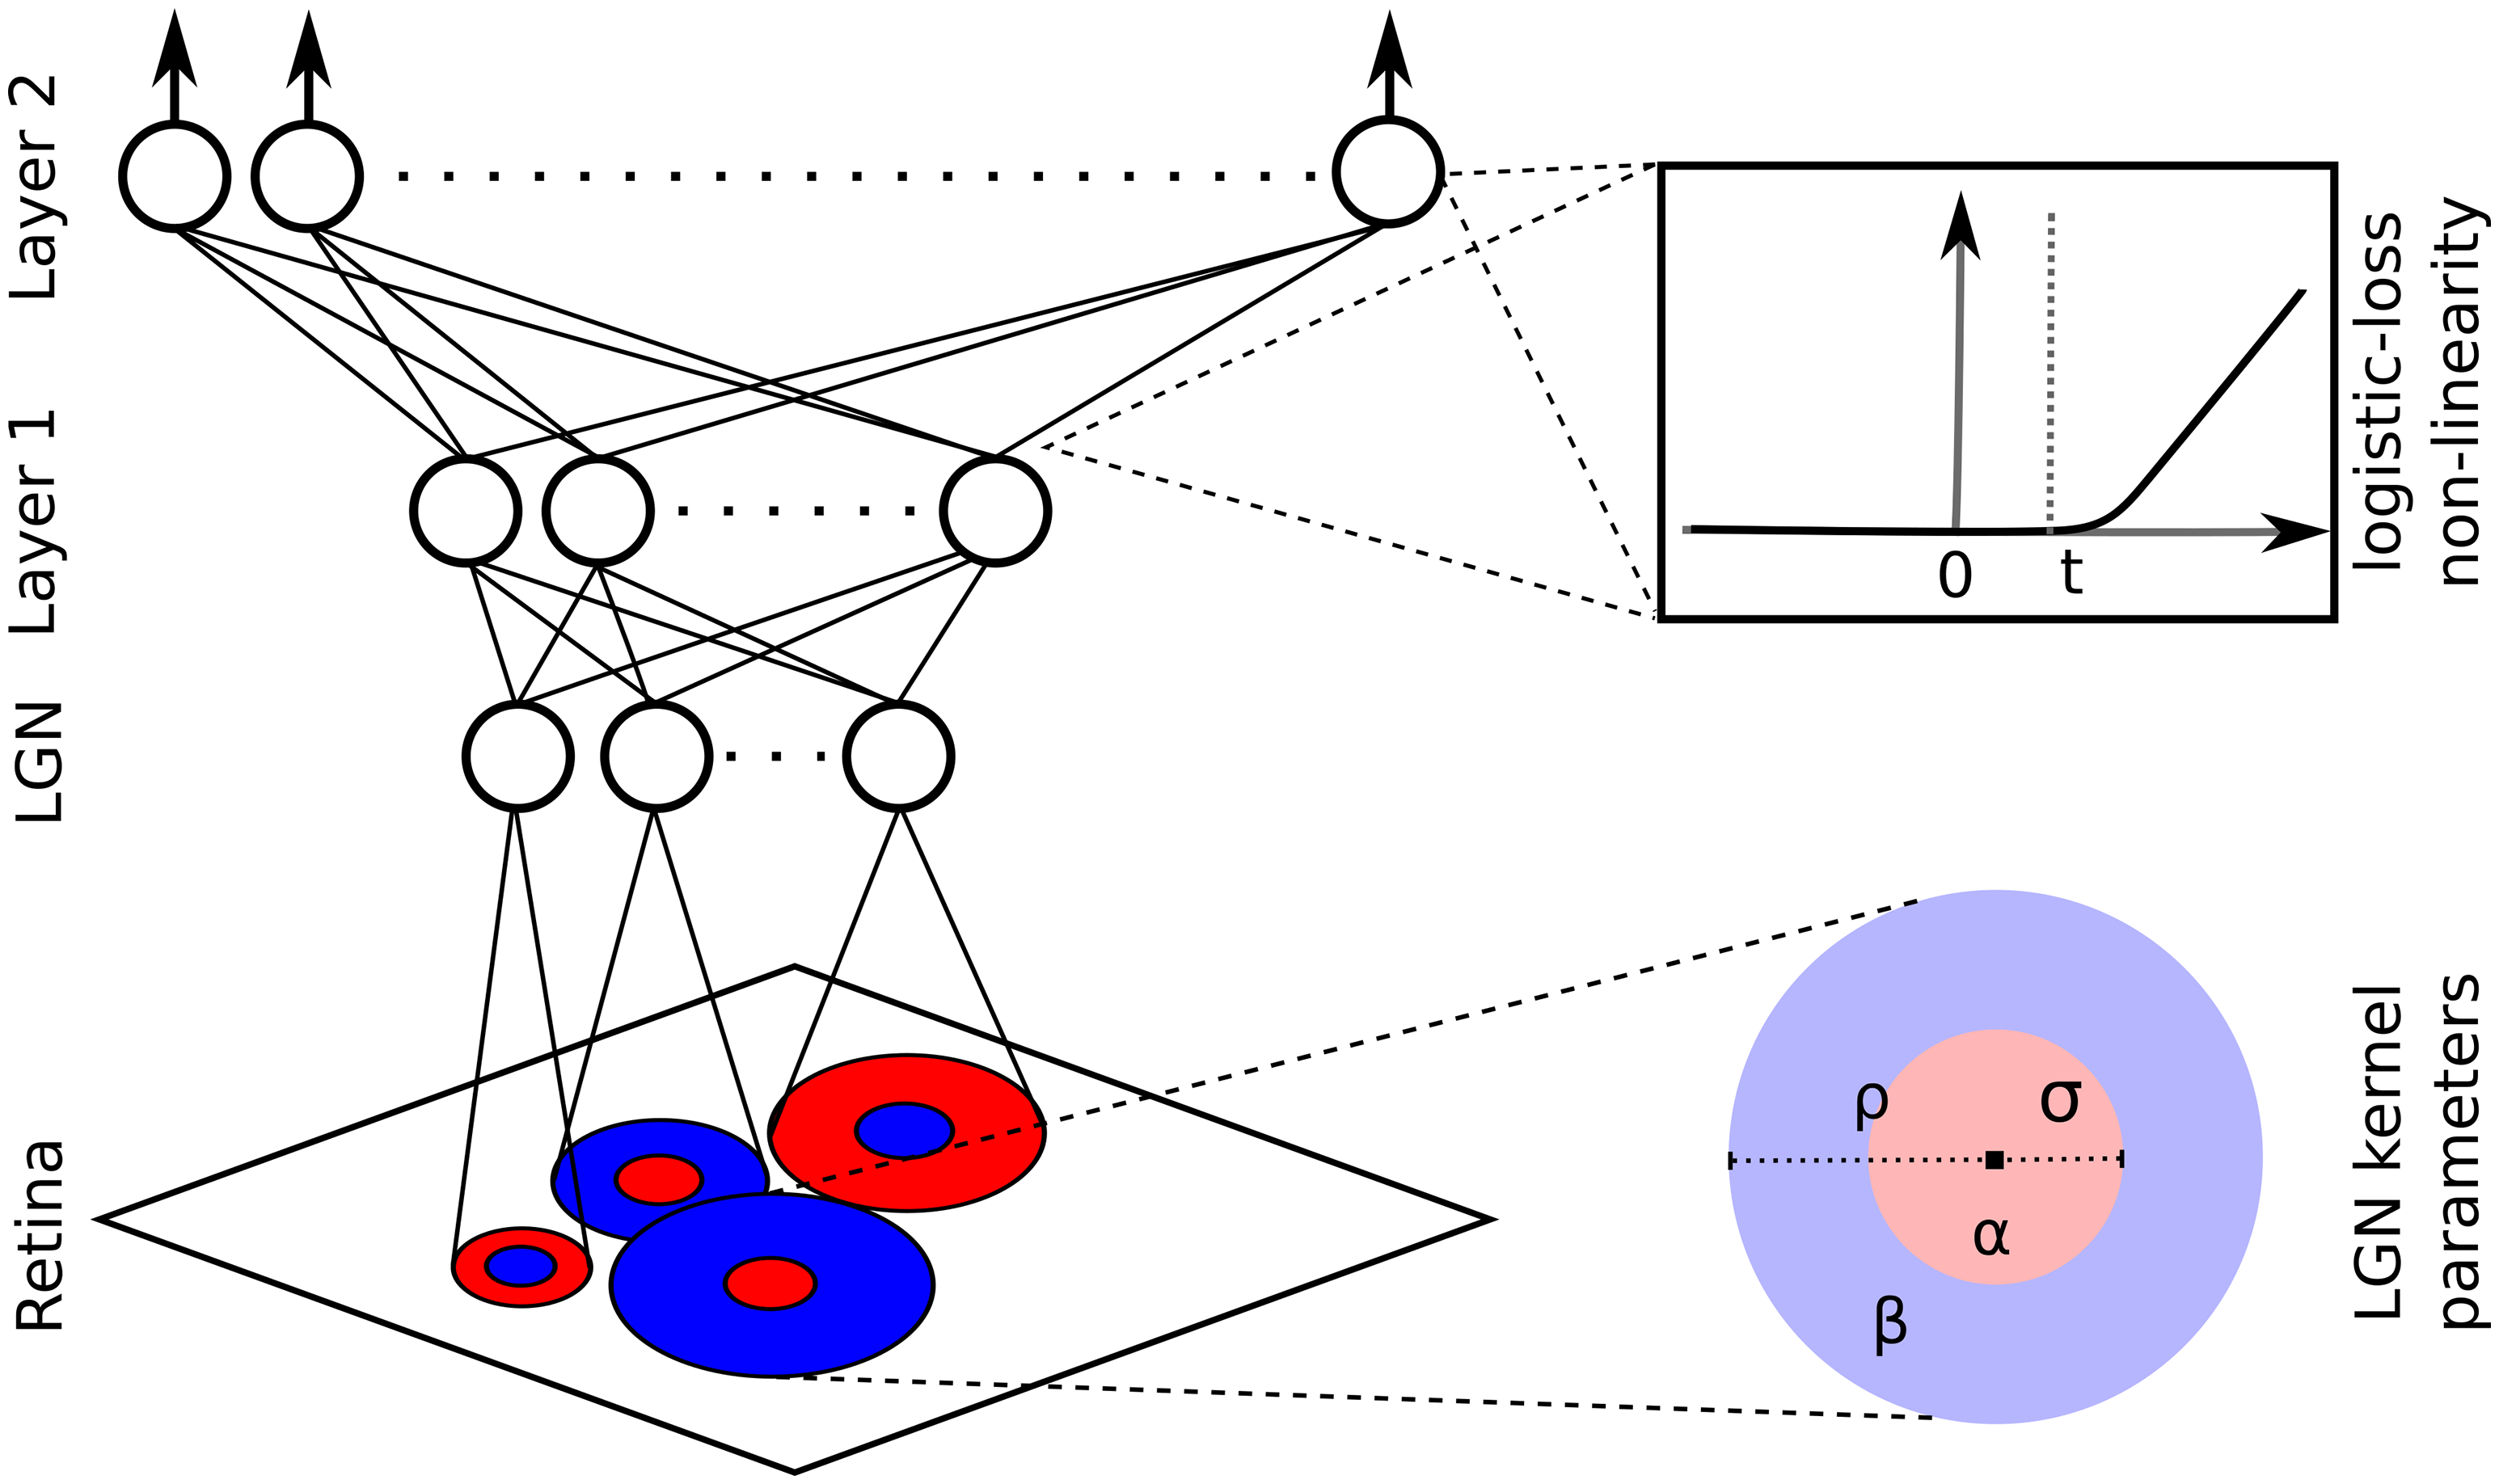
\includegraphics[width=1\textwidth]{../figures/02_HSM}
    \caption[HSM model architecture]{Three layer architecture of HSM model and corresponding neural sections. Figure was adopted from \citep{antolik}.}
    \label{fig:2.1}
\end{figure}

\subsection{Training regime}\label{ch:2.1.3}

The published model was trained using a Newton Conjugate-Gradient algorithm\footnote{\href{https://docs.scipy.org/doc/scipy/reference/generated/scipy.optimize.fmin_tnc.html}{https://docs.scipy.org/doc/scipy/reference/generated/scipy.optimize.fmin\_tnc.html}.} with 100 epochs, each consisting of 10 000 evaluations maximum. The batch size for this optimiser is the entire dataset. In addition to the hard regularization provided by the parameterized filters of the DoG layer, all parameters - of the weights of DoG layer and both fully connected layers - were kept within predefined bounds by the optimiser throughout the fitting. These bounds were also used for random initialization of the parameters, during which values were drawn from uniform distributions with corresponding bounds. No other soft or hard regularization is present in the model. 

The reported values for the hidden layer size ratio and the number of DoG filters hyperparameters were found empirically using two one-dimensional searches through the parameter space.

\section{Klindt et al. and the separable layer}\label{ch:2.2}

In \citeyear{klindt} \citeauthor{klindt} published a paper \textit{Neural system identification for large populations separating “what” and “where”} that explored deep convolutional neural networks in the context of V1 neural data. It specifically focused on the estimation of individual neurons’ receptive field locations through a novel approach to readout layer\footnote{Readout layer is the first fully connected layer after a set of convolutional layers.} factorization, in an effort to allow effective fitting of thousands of neurons on relatively little data simultaneously. In addition to artificial data, it was also evaluated on the same dataset as \cite{antolik} where it achieved state of the art results\footnote{For results refer to \refsection{ch:4.1.2}.}, improving on \cite{antolik}

\subsection{Architecture}

The what/where model consists of two parts, feature space and receptive fields (Fig. \ref{fig:2.2}). The feature space is a cascade of - in the variant for \citeauthor{antolik} dataset - 3 convolutional layers, each followed by a batch normalisation\footnote{\citep{2015arXiv150203167I}} and a SoftPlus activation function. The convolution layers have 48 feature maps per each layer, with the first one having 13 pixel and the other two 3 pixel kernels. In addition, the convolution layers feature two types of soft regularizations. A Laplacian regularizations to ensure smoothness of the filters and an L2 based group sparsity regularization\footnote{For a definition, please refer to the original paper \citep{klindt}.} to encourage filters to pool from only a small set of feature maps in the previous layer.

\begin{figure}[h]
    \centering
    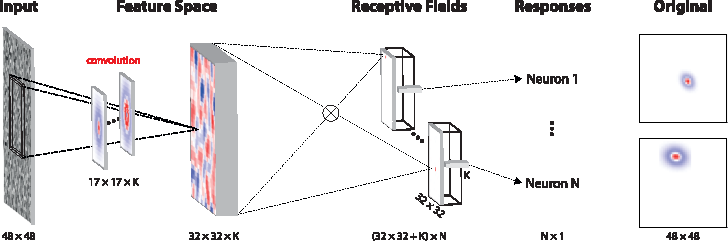
\includegraphics[width=1\textwidth]{../figures/02_fig2}
    \caption[klindt et al. model]{Architecture of \citeauthor{klindt} model, consisting of convolution layers and a factorized readout layer. Figure was adopted from \citep{klindt}.}
    \label{fig:2.2}
\end{figure}

The receptive field consists of a single instance of a specific readout layer (further referred to as the separable layer). It is a fully connected layer factored into two masks per each output neuron. First mask, with dimensionality \texttt{feat\_space\_output\_spatial\_dims}, selects the input locations the output neuron will use, in essence its receptive field - the “where”. The other, with dimensionality of \texttt{feat\_space\_output\_channels}, determines what channels of the feature space at each of the locations will make the neuron’s output - its “what”. This factorization achieves two things. It decreases the number of free parameters, from \texttt{spatial\_dims}$*$\texttt{channels} to \texttt{spa\-tial\_dims}$+$\texttt{channels} but also enables more direct interpretability of the parameters. Comparing the “what” masks, for example, allows us to identify similar cell types. Both masks feature L1 regularization to encourage sparsity.

The model was trained using ADAM optimiser and early stopping on 20/80 training set split. Reported hyperparameters, such as the number and size of convolution filters, were found and cross-validated using grid search for each region.

\section{Related works}\label{ch:2.3}
To provide some background, this section lists a few related works that are relevant to V1 system identification but are not directly used or in any way referenced by our experiments. Specifically, we will introduce a few convolutional architectures, as they have seen an increase in usage for V1 modeling, similarly as they have taken over classical computer vision\footnote{Even though they are slowly being superseded by attention/transformer-based networks: \citep{2019arXiv190605909R}, \citep{2019arXiv190409925B}), \citep{dosovitskiy2020image}.}.

\subsection{Neural convolutional models}
\cite{ecker} inspired by aforementioned \cite{klindt}, further explored convolutional architectures. In addition to the \citeauthor{klindt}’s observation that many neurons of early visual processing are similar but only have their receptive fields at different locations, \citeauthor{ecker}’s model leveraged the fact that even more V1 neurons are functionally the same, if we assume not only arbitrary receptive field positions but also arbitrary orientations. Based on the same two parts, 3 convolutional layers architecture introduced by \citeauthor{klindt}, their model used Group equivariant convolutions \citep{2016arXiv160207576C} instead of traditional convolution layers.

Tackling a similar problem from a different angle, \cite{Walke506956} introduced a convolutional architecture, where the readout locations - representing the receptive fields of output neurons - are modulated by a shifter side network based on eye movement data. In addition, the neural outputs are further adjusted by a second side network using behaviour data (running state, pupil dilation), trying to incorporate extra-retina sources of LGN and further downstream stages of visual processing. For the core network, the model used a three layer convolutional cascade followed by a neuron specific linear readout stage. 

\subsection{Transfer learning}

Motivated by the observation that lower parts of the visual pathway can be seen analogous to early layers of classical object recognition neural networks, \cite{10.1371/journal.pcbi.1006897} explored transfer learning within the domain of V1 system identification. Their proposed architecture used 16 feature maps\footnote{The output of one filter of a convolutional layer given a specific input.} from the initial section of an on-image-classification-dataset already trained VGG-16 network \citep{VGG16} and then fitted per output neuron readout layer on neural data. This approach managed to achieve parity with a 3 convolutional layer CNN architecture trained entirely on neural data, while requiring a smaller training dataset.
